\documentclass{article}
\usepackage{url,Sweave}
%\VignetteIndexEntry{Brief history of path analysis}
\newcommand{\R}{{\normalfont\textsf{R}}{}}
\newcommand{\car}{\texttt{car}}
\newcommand{\effects}{\texttt{effects}}
\newcommand{\code}[1]{\texttt{#1}}
\usepackage[authoryear,round]{natbib}
\bibliographystyle{plainnat}

<<echo=FALSE>>=
options(width=80, digits=4, useFancyQuotes=FALSE, prompt=" ", continue=" ")
@

\title{A (very) brief history of path analysis \&{} Structural Equation Modeling}
\author{Timothy C. Bates\footnote{Department of Psychology, University of Edinburgh}}
\date{\today}
\begin{document}
\maketitle

\begin{abstract}
Structural Equation Modeling has a fascinating history, at the intersection of sciences such as genetics, philosophical questions such as causality, and the development of statistics. It is a very recent development (Sewall Wright's seminal work was only published in 1918 \citet{Wright1918}), and a radical departure, proposing as it does a graphical method for thinking about causation. This small paper provides some insight into these developments, and pointers to further reading.
\end{abstract}

\section{Appendix 1: A (very) brief history of path analysis and SEM} % (fold)
\label{sec:sec_appendix1}

Early in the last century, \citet{Wright1918} developed path analysis as a tool for modeling sources of variance--initially in a dataset of rabbit skeletal dimensions. Wright saw that ``\emph{The correlation between two variables can be shown to equal the sum of the products of the chains of path coefficients along all of the paths by which they are connected}'' \citep[p. 115]{Wright1920}. This insight lead Wright to propose a graphical method for thinking about causation which, he realized, could be generalized, enabling decomposition of associations among variables into modeled sources of variance: for instance environmental and genetic variance \citep{Wright1920}. His now-classic and influential path diagram from this paper is shown in Figure~\ref{figure:SewellWrightpiebald}.

\begin{figure}[htbp]
	\centering
  	\includegraphics[scale=0.25]{figs/SewelWright1920.png}
	\caption{The first path diagram, showing inheritance of piebald pattern in the Guinea Pig \citep{Wright1920}.}
	\label{figure:SewellWrightpiebald}
	% Figure~\ref{figure:SewellWrightpiebald}
\end{figure}

Surprisingly, this graphical method for thinking about causation, so well suited to variables measured with error, and to modeling of multiple outcomes and causal effects, where each variable may have multiple influences, lay fallow for 30 years until its importance was recognized once more in the 1960s and 1970s by a sociologist \citep{Duncan1996} and an economist \citep{Goldberger1971} who alerted their fields to the value of structural equation modeling. Importantly, this alert was accompanied by the advent of accessible and powerful computer resources, which made practical widespread use of such models and saw the emergence of application-level software support for structural equation modeling \citep[]{Joreskog1969a}. Enhanced by developments continuing to the present day, modern extended SEM allows causal modeling of data \citep{Pearl2009}, including continuous, ordinal and binary measures. 

Models of these data types can include not only measured variables, but unmeasured ``latent'' constructs and relations among multiple variables. These measurement and structural models are conveniently represented graphically, with a standard set of symbols consisting of boxes (measured or manifest variables), circles (latent, or unmeasured variables), triangles (means) and diamonds (subject-specific or definition variables) and connections or paths among these objects consisting of single-headed directional paths representing directed causal influences, and two-headed curved paths representing covariance between variables. The model, once run, yields parameter estimates of these paths that may be extracted, used to form scores, plotted, etc. Models themselves can be compared using goodness of fit indicators. In Figure~\ref{figure:mpg}, a simple model shows how one might begin to graphically model the relationship of fuel efficiency (miles per gallon) of a car to its weight and the size (cubic capacity) of its engine in a path diagram. In this model, engine size and weight correlate (.89) and negatively influence mpg.

\begin{figure}[htbp]
	\centering
  	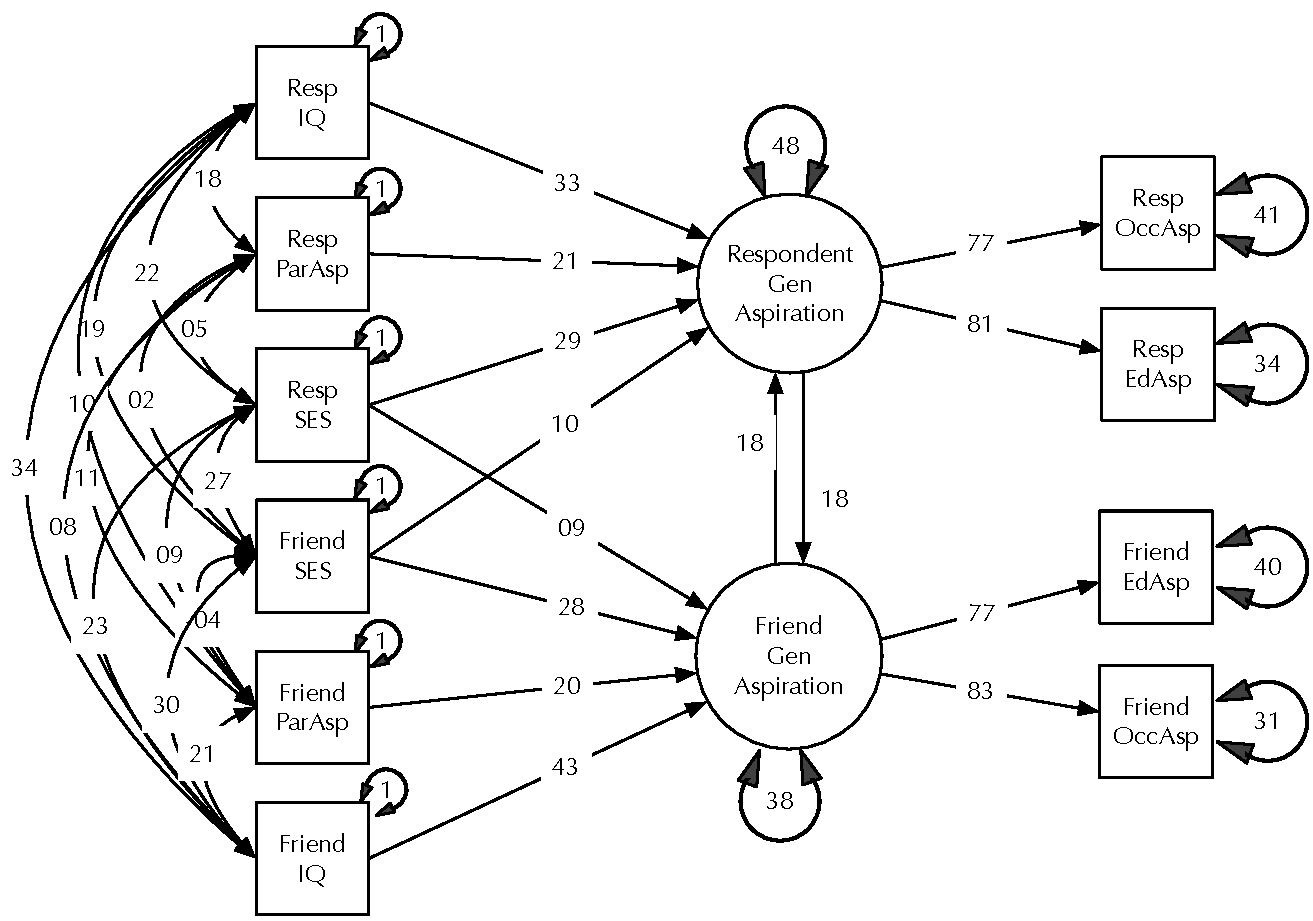
\includegraphics[scale=0.60]{figs/Duncan.pdf}
	\caption{A model of fuel economy in terms of vehicle weight and engine capacity .\label{figure:Duncan}}
	% Figure~\ref{figure:DuncanPeer}
\end{figure}

% section sec_appendix1 (end)